ترتیب اولیه دستورات به این صورت است:

\setLTR
\begin{lstlisting}
I1:     lw      R1, 0(R2)       ; R1 ← Memory[R2]
I2:     addi    R1, R1,     1   ; R1 ← R1+1
I3:     sw      R1, 0(R2)       ; Memory[R2] ← R1
I4:     addi    R2, R2,     8   ; R2 ← R2+8
I5:     addi    R4, R4,     -1  ; R4 ← R4-1
I6:     bne     R4, R0,     I1  ; branch if R4!=0
\end{lstlisting}
\setRTL

\subsubsection*{الف}
باید جایگاه
$I_5$
را طوری تغییر بدهیم که حداقل 2 مرحله زودتر از 
$I_6$
اجرا شود.

\setLTR
\begin{lstlisting}
I1:     lw      R1, 0(R2)       ; R1 ← Memory[R2]
I5:     addi    R4, R4,     -1  ; R4 ← R4-1
I2:     addi    R1, R1,     1   ; R1 ← R1+1
I3:     sw      R1, 0(R2)       ; Memory[R2] ← R1
I4:     addi    R2, R2,     8   ; R2 ← R2+8
I6:     bne     R4, R0,     I1  ; branch if R4!=0
\end{lstlisting}
\setRTL

\subsubsection*{ب}
در این بخش ما دستوری را بعد از 
$I_6$
قرار می‌دهیم که هر بار اجرا شود و ارتباطی با شرط پرش نداشته باشد.

\setLTR
\begin{lstlisting}
I1:     lw      R1, 0(R2)       ; R1 ← Memory[R2]
I5:     addi    R4, R4,     -1  ; R4 ← R4-1
I2:     addi    R1, R1,     1   ; R1 ← R1+1
I3:     sw      R1, 0(R2)       ; Memory[R2] ← R1
I6:     bne     R4, R0,     I1  ; branch if R4!=0
I4:     addi    R2, R2,     8   ; R2 ← R2+8
\end{lstlisting}
\setRTL

\subsubsection*{ج}

با توجه به خواسته سوال، جدول زیر را تشکیل می‌دهیم:
\setLTR

$ \ \ 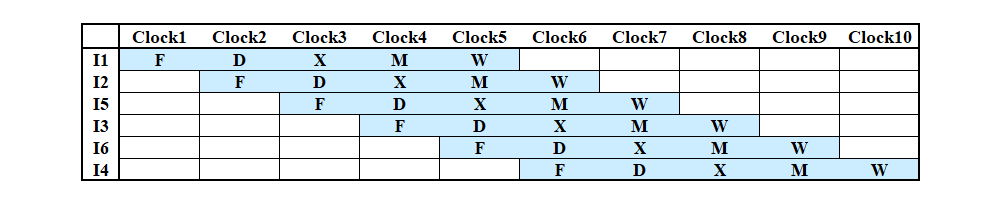
\includegraphics[width=1\linewidth]{figs/1.png}$

\setRTL

اگر فقط یک بار این حلقه اجرا شود، در مجموع 10 کلاک زمان می‌برد، اما اگر چندین بار این حلقه تکرار شود، تقریبا به تعداد حلقه‌ها نیاز به کلاک داریم.



